This is the seventh in a series of tutorials on the use of the
\gwendolen\ programming language.  This tutorial covers the
\gwendolen\ Reasoning Cycle, looks at some simple ways to use a Java
Debugger to debug \gwendolen\ programs and sets a more significant
programming challenge than previous
tutorials.\index{Gwendolen}\index{reasoning
  cycle}\index{Gwendolen!reasoning cycle}\index{debugging!with a Java
  debugger}\index{Gwendolen!debugging} 

Files for this tutorial can be found in the \texttt{mcapl}
distribution in the directory 
\begin{quote}
\texttt{src/examples/gwendolen/tutorials/tutorial7}.
\end{quote}

\section{The \gwendolen\ Reasoning Cycle}\index{reasoning cycle}\index{Gwendolen}\index{Gwendolen!reasoning cycle}

The execution of a \gwendolen\ agent is governed by a \emph{reasoning
  cycle}.  This is a set of stages the agent passes through, each
stage is governed by a set of rules and the agent may choose one to
execute in that stage.  The reasoning cycle is shown in
figure~\ref{fig:reasoning_cycle}\index{Gwendolen}\index{reasoning
  cycle}\index{Gwendolen!reasoning cycle} 
\begin{figure}
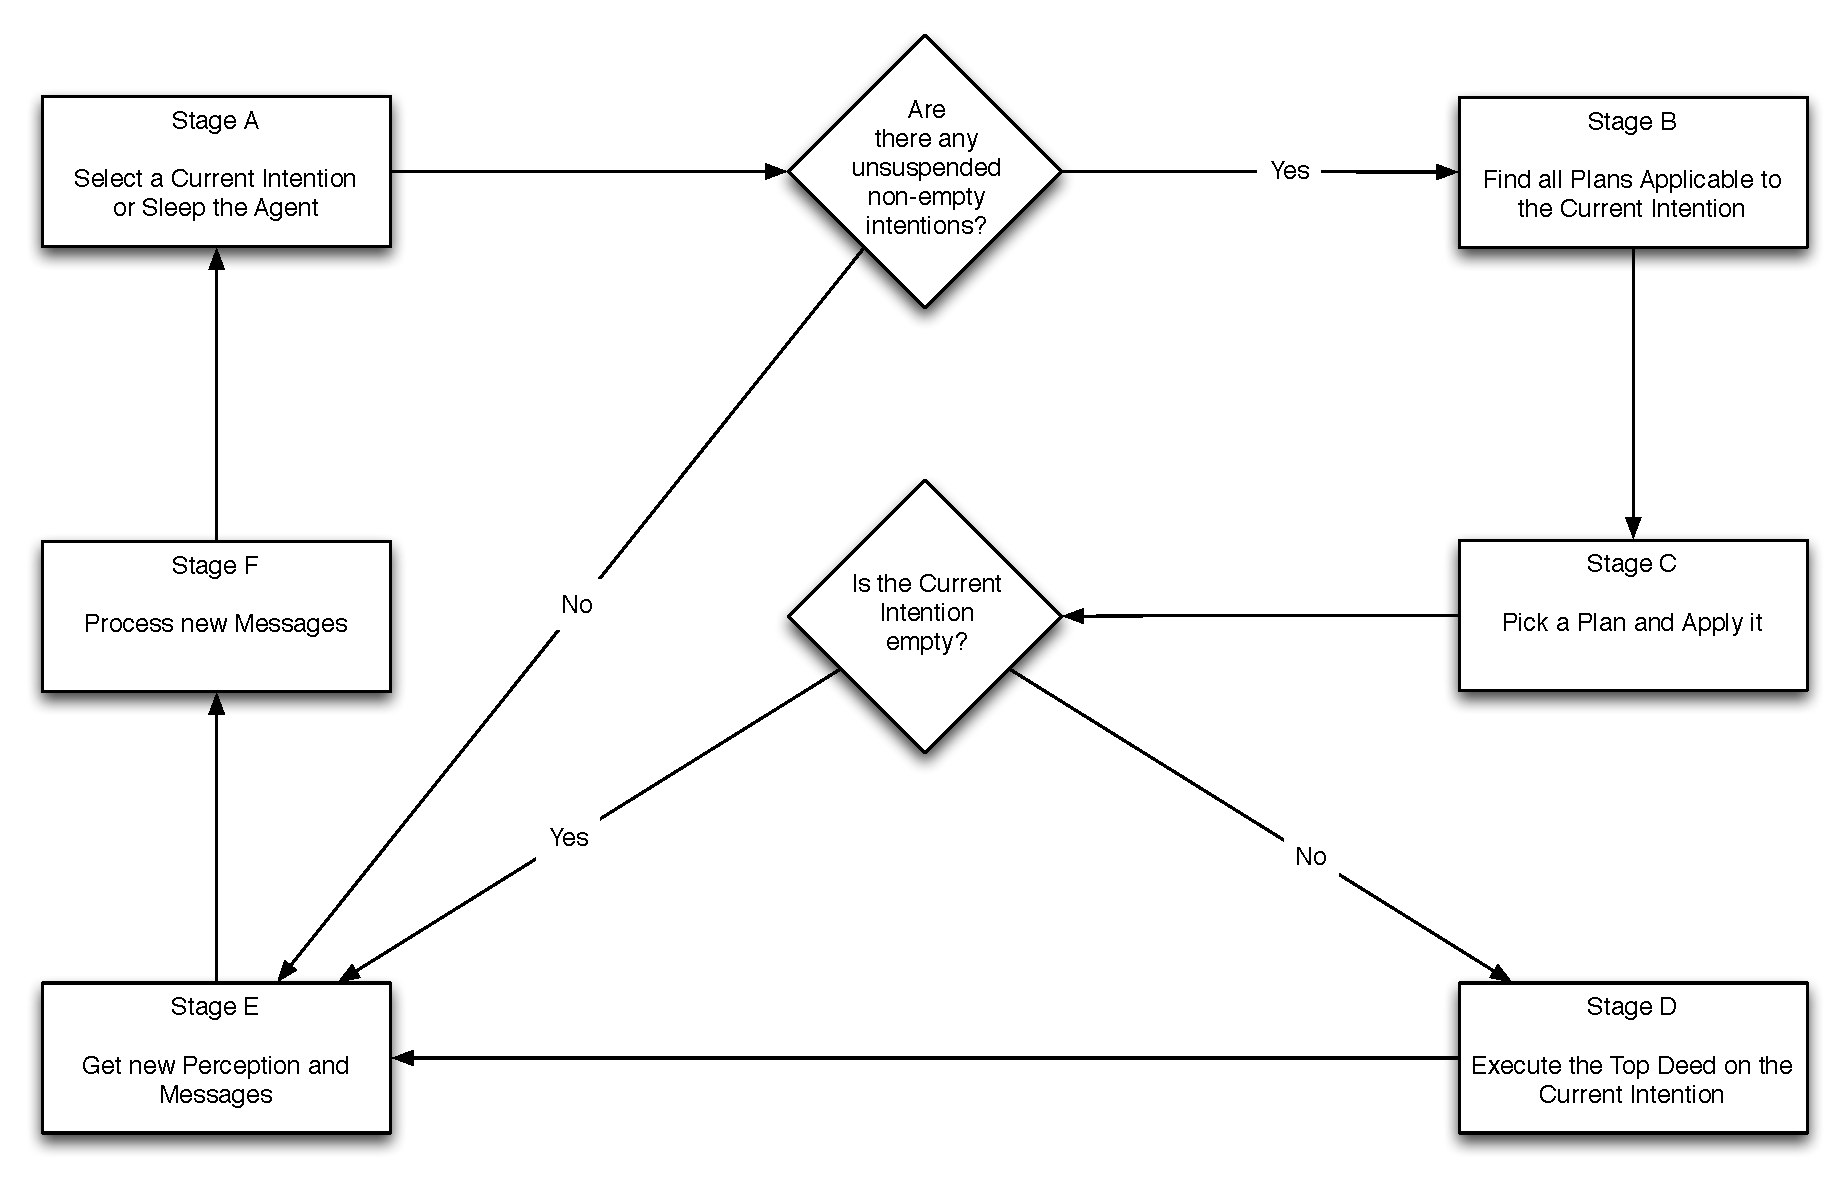
\includegraphics[width=\textwidth]{images/ReasoningCycle.pdf}
\caption{The \gwendolen\ Reasoning Cycle}
\label{fig:reasoning_cycle}
\end{figure}
\begin{description}
\item[Stage A]
A \gwendolen\ agent starts execution in stage A.  In this stage the
agent selects an intention to be the current
intention\index{intention}\index{intention!current}.  \gwendolen\ will
cycle through the set of intentions ignoring any that are
suspended\index{intention!suspension} until the current intention is
locked\index{intention!locking} in which case it will be reselected.
If there are no unsuspended intentions \gwendolen\ will sleep the
agent\index{sleeping}.  In multi-agent contexts this means the agent
will not do anything until \gwendolen\ detects that something has
changed which may mean the agent now has something to do.  In single
agent contexts the program stops when the agent sleeps.  At this stage
\gwendolen\ also cleans up any empty
intentions.\index{Gwendolen}\index{intention!empty} 
\item[Stage B]
The system generates all possible plans for the current intention - if
the intention has already been planned then these are simply to
continue processing the intention.  If the agent can't find a plan
then it deletes the intention unless it has been triggered by a goal
in which case it registers that there is a problem with the goal and
generates a
warning.\index{plan}\index{plan!generation}\index{goal}\index{goal!problem} 
\item[Stage C]
\gwendolen\ has a list of plans.  It selects the first one in the list
and applies it to the current
intention.\index{plan}\index{intention}\index{Gwendolen} 
\item[Stage D]
\gwendolen\ executes the top deed on the intention.  This might be
taking an action, adding or removing a goal, adding or removing a
belief, locking or unlocking the intention or suspending the intention
using ``wait
for''.\index{intention}\index{intention!execution}\index{deed}\index{deed!top} 
\item[Stage E]
\gwendolen\ requests that the agent's environment send it a list of
\emph{percepts} (things the agent can detect) and messages.  The
messages are stored for processing in the agent's inbox.  The percepts
are compared with the agent's beliefs.  If a percept is new then an
intention is created to add a belief corresponding to the percept.  If
a previous percept can no longer be perceived then an intention is
created to delete the
belief.\index{perception}\index{communication}\index{message} 
\item[Stage F]
The agent sorts though its inbox and converts the messages into new
intentions.\index{message!converted to intention}\index{Gwendolen} 
\end{description}

\begin{sloppypar}
The actual code for the reasoning cycle can be found in
\texttt{gwendolen.semantics.GwendolenRC}\index{GwendolenRC
  (class)}\index{reasoning cycle}.  Each of the various rules that can
be used in in a stage is a java class and they can all be found in the
package \texttt{ail.semantics.operationalrules}\index{operationalrules
  (package)}. 
\end{sloppypar}

\section{Using Java Debuggers to Debug \gwendolen\ programs}\index{debugging}\index{debugging!with a Java debugger}\index{Gwendolen!debugging}

Since the \gwendolen\ reasoning cycle\index{reasoning cycle} is
implemented in \java\ it is possible to use a \java\ debugger to debug
\gwendolen\ programs.  In particular it can be useful to use a
\java\ debugger to step through a \gwendolen\ program one stage of the
reasoning cycle at a time watching to see how the state of the agent
changes at each
stage.\index{Gwendolen}\index{debugging}\index{debugging!with a Java
  debugger}\index{Gwendolen!debugging} 

It is outside the scope of these tutorials to explain the use of
\java\ debuggers.  There are many out there and one is built into most
IDE's including Eclipse.\index{Java} 

In our experience it is particularly useful when debugging in this way
to place breakpoints in the
\java\ \texttt{ail.semantics.AILAgent}\index{AILAgent (class)} class
which is the generic class supporting agents in the Agent
Infrastructure Layer\index{AIL} (upon which \gwendolen\ is built).  In
particular \texttt{ail.semantics.AILAgent} has a method called
\texttt{reason}\index{AILAgent (class)!reason} which controls looping
through an agent's reasoning cycle\index{reasoning cycle}.  We
recommend placing such a break point either after \texttt{while(!
  RC.stopandcheck())} which is the top level loop through the
reasoning cycle or at \texttt{rule.apply(this)} which is the moment
that the outcome of a rule is calculated. 

\begin{sloppypar}
\paragraph{Exercise} Find a \java\ debugger (e.g., the one shipped
with Eclipse) and discover how to set breakpoints using the debugger.
Set a breakpoint at \texttt{rule.apply(this)} in the \texttt{reason()}
method in \texttt{ail.semantics.AILAgent} (you can find this in the
\texttt{src/classes/ail/semantics} directory).  Run one of your
programs with this breakpoint in place and see what happens and
experiment in seeing what information you can discover about the agent
state.\index{debugging!exercises}\index{AILAgent
  (class)}\index{AILAgent (class)!reason} 
\end{sloppypar}

\section{Programming Exercise}\index{Gwendolen}\index{Gwendolen!exercises}
This is a fairly major programming exercise using the
\gwendolen\ constructs you have already been introduced to.  As usual
a sample solution can be found in the \texttt{answers} subdirectory
for \texttt{tutorial7}. 

In \texttt{examples/gwendolen/tutorials/tutorial7} you will find a new
environment,
\texttt{SearchAndRescueDynamicEnv.java}\index{SearchAndRescueDynamicEnv
  (class)}.  This extends the previous search and rescue example so
that the environment may change with the agent directly taking any
action.  The following describes the environment. 

The environment consists of a 5x5 grid of squares.  The squares in the
grid are numbered from (0, 0) (bottom left) to (4, 4) (top right).  On
this grid are 
\begin{itemize}
\item Exactly four humans which may start in any square on the grid.
  Some of these humans may be {\bf injured}. 
\item Exactly one robot which starts in the bottom left corner of the grid.
\item Up to four buildings which may appear in any square on the grid.
\item Up to four bits of rubble which may appear in any square on the
  grid.  Any human on the same square as some rubble at the start is
  {\bf injured} and is hidden under the rubble. 
\end{itemize}

At any point the following may happen:
\begin{itemize}
\item A human who is not {\bf injured}, {\bf in a building}, or has
  been {\bf directed to leave} the area may move one square in any
  direction. 
\item A building may collapse into rubble.
\end{itemize}

The robot  has the following actions available to it:
\begin{description}
\item[back\_left] If possible the robot will move one square diagonally down the grid and to the left.  If not possible the robot will do nothing.
\item[back] If possible the robot will move one square down the grid.  If not possible the robot will do nothing.
\item[back\_right] If possible the robot will move one square diagonally down the grid and to the right.  If not possible the robot will do nothing.
\item[left] If possible the robot will move one square to the left.  If not possible the robot will do nothing.
\item[right] If possible the robot will move one square to the right.  If not possible the robot will do nothing.
\item[forward\_left] If possible the robot will move one square diagonally forward in the grid and to the left.  If not possible the robot will do nothing.
\item[forward] If possible the robot will move one square forward in the grid.  If not possible the robot will do nothing.
\item[forward\_right] If possible the robot will move one square diagonally forward in the grid and to the right.  If not possible the robot will do nothing.
\item[lift\_rubble] If the robot is not currently holding rubble then it will pick up one piece of rubble in the square revealing anything underneath it.
\item[drop\_rubble] If the robot is holding rubble then it will drop it in the current square, injuring and concealing any humans if they are in the square.
\item[assist\_human] If there is an injured human in the square then the robot treats them with first aid.  After this the human is not injured.
\item[direct\_humans] If there are any humans in the square then the robot tells them to leave the area immediately.
\item[check\_building] If there is a building in the square then the robot looks inside it to see if there is a human there.
\item[Other Actions] Other standard actions such as \texttt{print} and \texttt{do\_nothing} are also available.
\end{description}

The robot may perceive the following things:
\begin{description}
\item[holding\_rubble] perceived if the robot has rubble in its hands.
\item[rubble(X, Y)] perceived if the robot sees some rubble in square (X, Y).  The robot can see the square it is in and one square in each direction.
\item[building(X, Y)] perceived if the robot sees a building in square (X, Y).  The robot can see the square it is in and one square in each direction.
\item[injured\_human(X, Y)] perceived if the robot sees an injured human in square (X, Y).  The robot can see the square it is in and one square in each direction.
\item[uninjured\_human(X, Y)] perceived if the robot sees an uninjured human in square (X, Y).  The robot can see the square it is in and one square in each direction.
\end{description}

The following also hold true:
\begin{itemize}
\item If a human is {\bf in a building} when it collapses then they will be {\bf injured} and concealed by the rubble.
\item If a human is {\bf in a building} then the robot can not see them unless it checks the building.
\end{itemize}

Humans exhibit the following behaviour:
\begin{itemize}
\item {\bf injured} humans do not move.
\item {\bf directed} humans move diagonally down and left until they leave the grid.  They do not enter buildings.
\item If a human is not {\bf directed} and finds itself in a square with a building then it will enter the building and stay there.
\item Humans which are not {\bf injured}, {\bf directed} or {\bf in a building} will move at random around the grid.
\end{itemize}

\subsection{Recording and Replaying \ail\ Programs}\index{record random execution}\index{replay execution}
We will cover recording and replaying \ail\ programs in more detail in
a later tutorial.  However some of the challenges from this tutorial
will arise because of the difficulty in reproducing a specific
sequence of events in the environment.  In the \ail\ configuration
file you can put the line 

\begin{verbatim}
ajpf.record = true
\end{verbatim}

\index{ajpf.record}
This will record the sequence of events that occur in the environment
(and store them in a file called \texttt{record.txt} in the folder
\texttt{records}).  If you want to \emph{replay} the last recorded run
of the problem then replace 

\begin{verbatim}
ajpf.record = true
\end{verbatim}

with \index{ajpf.replay}

\begin{verbatim}
ajpf.replay = true
\end{verbatim}

\subsection{Exercise}
Write a \gwendolen\ program that will get the robot to search the grid
until all humans have been found, assisted if injured, and directed to
leave.\index{Gwendolen} 

